\section{Introduction}
\label{section:s_introduction}

	\subsection{What is SpyGlass?}
		SpyGlass is an application primarily designed to visualize sensor networks on 
		a screen. It displays a set of sensor nodes at their location on a map, as well 
		as arbitrary data sent by the nodes, e.g. connectivity status between nodes or 
		aggregated data collected by the nodes’ sensors.
	
		The SpyGlass application itself is a framework, designed to be extendable by 
		plugins that visualize arbitrary things. In fact, all visualization and data aggregation
		that is currently done, is done by a set of bundled plugins, each fulfilling a 
		certain functionality. As said before, the primary focus of SpyGlass is the
		visualization of a set of sensor nodes, forming a network. However, SpyGlass can
		also be used in other, nearly arbitrary scenarios, where packet based communication 
		is used. This is because visualization is done based on network packets, 
		which represent statistical, structural or any other arbitrary data, sent by the 
		nodes to the SpyGlass application. Those packets are then dispatched to the 
		various plugins, which in turn, interpret the packet, draw things onto the screen 
		when appropriate and aggregate data contained in the packet. The whole range of visualization 
		opportunities, delivered by the currently bundled plugins, will be explained in 
		this document in the various chapters describing the bundled plug ins.
		
		SpyGlass bases on the requests given by the Institute of Telematics (ITM) of 
		the University of Lübeck and was developed by Daniel Bimschas, Sebastian 
		Ebers, Dariush Forouher and Oliver Kleine in the context of a case study for 
		professional product development.

	\subsection{Installation}
	
		\subsubsection{Prerequisites}
			The SpyGlass application is available in two different versions. One is a plugin 
			for the iShell \footnote{see http://www.coalesenses.com/index.php?page=ishell}
			software, the other is a standalone version. For both versions, a 
			Java Runtime Environment (version 6.0 or newer) is necessary. For the iShell 
			version one needs a platform that is supported by iShell, which is currently 
			Windows and Linux.

			Tested plattforms are:

			\begin{itemize}
			  \item Linux x86
			  \item Linux AMD64
			  \item Windows (32bit)
			  \item Mac OS X with 64bit JRE (experimentally)
			\end{itemize}

		\subsubsection{Build instructions}
		
			The Spyglass project is hosted on SourceForge.net
			(\url{http://sourceforge.net/projects/itm-spyglass}).
			
			You can check out it’s sources with a Subversion client from
			\url{https://itm-spyglass.svn.sourceforge.net/svnroot/itm-spyglass}.

			Spyglass can be used in two ways:

			\begin{itemize}
			  \item{Either as a standalone application or}
			  \item{as a plugin inside the iShell tool.}
			\end{itemize}

			Since Spyglass uses the SWT framework, one has to
			decide at compile-time which platform one wants to use.

			Building Spyglass is very easy. One does not need any external
			libraries besides a working Java SDK and "ant".
			The resulting jar files contain all needed libraries (via the
			One-JAR\tm  boot-mechanism) and are directly executable.

		\subsubsection{Building Spyglass as a standalone application}

			Just run one of

			\begin{verbatim}
			    $ ant standalone-linux
			    $ ant standalone-linux64
			    $ ant standalone-win32
			    $ ant standalone-osx
			\end{verbatim}

			depending on the platform you want to run Spyglass on.

			These commands will build the file \texttt{spyglass-XXX-standalone.jar}, where
			\texttt{XXX} stands for the chosen architecture.
			This jar file includes all necessary dependencies and can be run directly via

			\begin{verbatim}
			    $ java -jar spyglass-XXX-standalone.jar
			\end{verbatim}

		\subsubsection{Building iShell with Spyglass included as a plugin}

			To build iShell with SpyGlass plugin one needs to run one of the commands

			\begin{verbatim}
				$ ant ishell-linux
				$ ant ishell-linux64
				$ ant ishell-win32
				$ ant ishell-osx
			\end{verbatim}

			depending on the platform one wants to use.

			These commands will build the file \texttt{ishell-XXX-spyglass.jar}, where
			\texttt{XXX} stands for the chosen architecture.
			This jar files includes a version of iShell, the compiled Spyglass source
			and all libraries both applications depend on.

			Similarly, it can be run directly via

			\begin{verbatim}
				$ java -jar ishell-XXX-spyglass.jar
			\end{verbatim}

\section{Using SpyGlass}
	
	\subsection{The application interface}

		As mentioned before, there are two different ways to start SpyGlass. First one 
		can start the standalone application, secondly it is a plugin for iShell. For the 
		latter one must start iShell first and activate the SpyGlass plugin afterwards. 
		All screenshots included in this manual are taken from SpyGlass as an iShell 
		plugin.

		On the first start of SpyGlass with an empty configuration one can see the 
		following things (see figure \ref{pic:spyglass_first_appearance}):
		
		\begin{figure}[htb]
			\begin{center}
				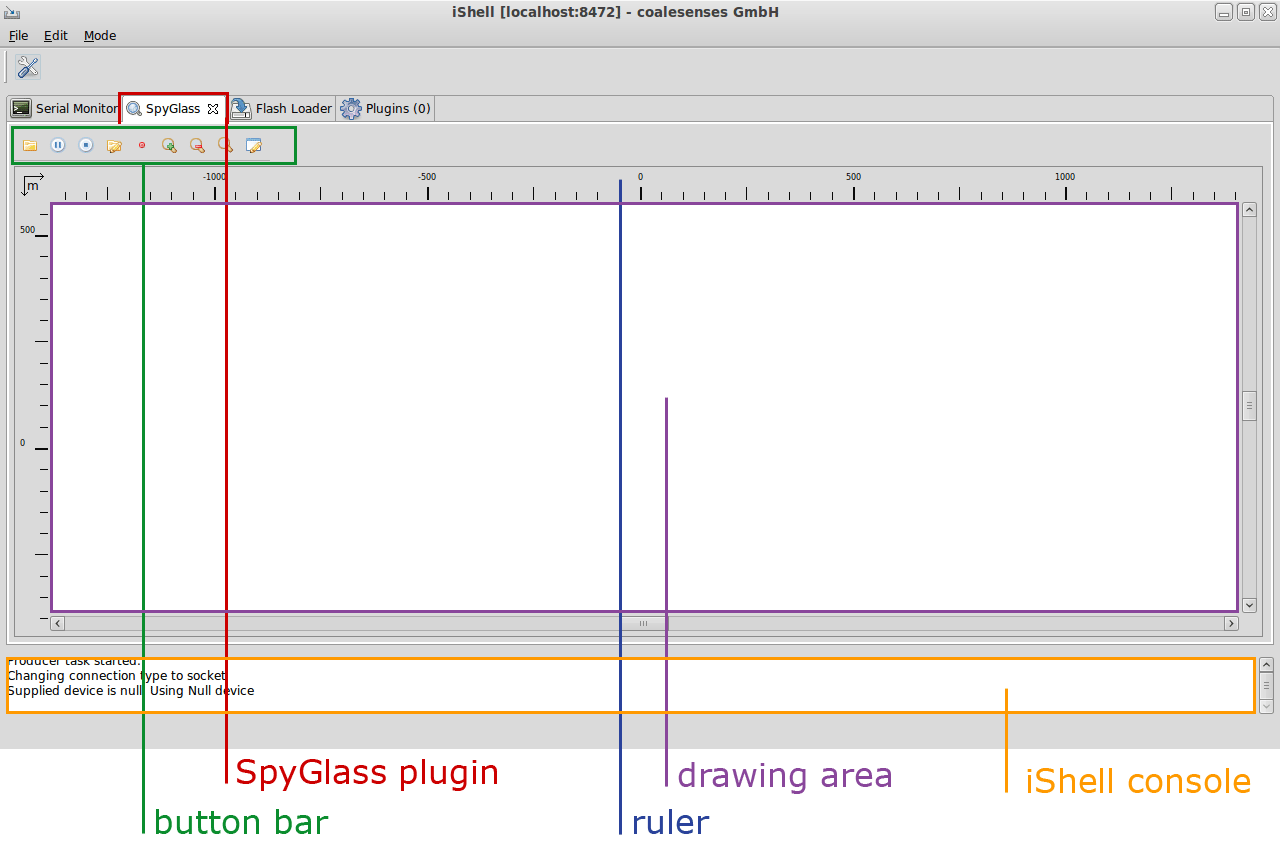
\includegraphics[width=13.2cm]{./pics/spyglass_first_appearance}
				\caption{Empty screen of the SpyGlass plugin for iShell}
				\label{pic:spyglass_first_appearance}
			\end{center}
		\end{figure}
		
		\begin{itemize}
			\item SpyGlass plugin\\
				As iShell contains of many plugins one must explicitly click on the tab for 
				the SpyGlass plugin to bring SpyGlass to the front.
			\item Button Bar\\
				all functions necessary to control the behaviour of SpyGlass can be found 
				here (check subsection \ref{ssec:buttons_behaviour} for a more detailed description).
			\item Drawing Area\\
				All visualization of the sensor network will take place here. The drawing 
				area shows a section of the whole sensor network. This section can be 
				enlarged by zooming out or downsized by zooming in. To change the 
				section to be shown on the drawing area without changing the zoom level, 
				one can either use the scrollbars on the bottom and on the right side of 
				the drawing area or hold the left mousebutton when the pointer is located 
				on the drawing area and move the mouse to the desired direction.
			\item Ruler\\
				The rulers’ labeling represents the current section of the drawing area 
				with respect to the real coordinates. Thus the labels of the ruler change 
				automatically, whenever the drawing area is either moved or if the zoom 
				level changes.
			\item iShell Console\\
				Logging console of the iShell application. iShell plugins print out log 
				messages to the console during runtime.
		\end{itemize}
		
		\paragraph{Differences in the standalone version}
			
			In the standalone version, all functionalities accessible by buttons in the button
			bar are also accessible via the windows’ menubar. Also, there is no iShell
			console in the standalone version.
			
	\subsection{Buttons and their behavior}
	\label{ssec:buttons_behaviour}

		\begin{figure}[htb]
			\begin{center}
				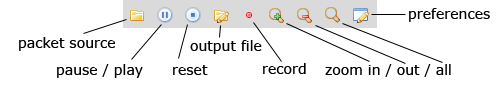
\includegraphics[width=11cm]{./pics/spyglass_buttons}
				\caption{SpyGlass buttons}
				\label{pic:spyglass_buttons}
			\end{center}
		\end{figure}

		In the following all buttons’ functionalities will be explained:
		
		\paragraph{Packet Source}
		  The button opens a dialog to define the current packet source. The source 
		  can either be iShell (through a TCP/IP socket connection) or a file. If 
		  the packet source is iShell, then the packets come from network. The real 
		  packet source (i.e. the packet source where iShell receives packets from)
		  must then be configured by setting the TCP/IP preferences of iShell.
		  
		  \emph{Please note:} In the standalone version of SpyGlass it is only possible to 
		  choose a file as packet source. For more information about how to generate 
		  such a file check the reference for the output file and record buttons.
			
		\paragraph{Pause / Play}
		  Clicking the pause button will stop the SpyGlass application delivering 
		  the sensor nodes’ packets to the various plugins currently active. By this, 
		  the visualization will freeze for the most parts as the plugins don’t receive 
		  new packets. However, some ob jects on the drawing area could disappear 
		  because they time out or they could move to another position for any 
		  reason (e.g. when using a SpringEmbedderNodePositioner, see subsection 
		  \ref{subsection:sep}). Also, plugins doing statistical calculations including
		  timing information, such as packets per second, will therefore display falsified
		  information during the time SpyGlass is paused.
		  
		  All new packets coming in during the time SpyGlass is paused, are queued. 
		  They are delivered sequentially after the play button has been clicked. The 
		  pause button toggles to a play button when it was clicked and vice versa.
				
		\paragraph{Reset}
		  Clicking the reset button will cause all active SpyGlass plugins to reset.
		  Resetting a plugin means that it forgets all aggregated data and removes
		  all drawings from the drawing area. You could say that, after all plugins
		  are reset, the application displays the same information as it displays
		  directly after startup. However, the configuration of plugin instances are kept.
				
		\paragraph{Output File / Record}
		  The record button is to start the recording of incoming packets. One must
		  specify a file, where the incoming packets will be written into. The file gets
		  the ending “.rec” and can be used later in both the standalone application
		  and the SpyGlass iShell plugin as a packet source. The record stops if one
		  clicks on the record button again. During the recording time, the button
		  is white. Otherwise it is red.
				
		\paragraph{Zoom In / Out / All}
		  The “+” and “-” buttons with the magnifier are pretty self-explanatory.
		  One zooms in (+) while the other zooms out (-). The third magnifier button
		  zooms exactly to the zoom level that all current network components
		  (nodes) are displayed on the drawing area.
		  
		  Additionally to the buttons, zooming can also be done with the scrollwheel
		  on the mouse, if the pointer is located on the drawing area.
				
		\paragraph{Preferences}
		  The button opens the preferences dialog, where you can configure the
		  SpyGlass application, as well as the spyglass plugin instances. All that is
		  described in detail from chapter 5 on.

